Et tre en et spesielt tilfelle av en rettet graf der hver node har inngrad 1 (med unntak av rota i treet). Vi ser på et eksempel:
\begin{figure}[h!]
\caption{Et lite binært tre}
\label{fig:tre}
\centering
~\\
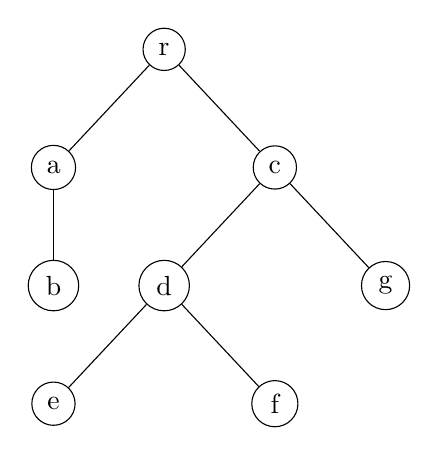
\begin{tikzpicture}[sibling distance=8em,
every node/.style = {shape=circle, draw, align=center}]

\node{r}
	child {node {a}
		child {node {b}}
	}
	child {node {c}
		child {node {d}
			child {node {e}}
			child {node {f}}
		}
		child {node {g}}
	};
\end{tikzpicture}
\end{figure}

\subsection*{Terminologi}
Vi skal se litt på ord og uttrykk for trær. Gjennomgående bruker vi treet i figur \ref{fig:tre} som eksempel

I figuren blir nodene tegnet som rundinger. For å betegne relasjonen mellom nodene bruker vi ofte familierelasjoner. Vi sier at $ e $ og $ f $ er \textbf{søsken}, $ d $ er \textbf{forelder} til $ e $, og $ e $ er \textbf{barn} av $ d $. Vi kan også si at $ g $ er \textbf{onkel} til $ f $, men dette er mindre vanlig, da vi sjeldent har bruk for å snakke om \say{onkelnoder}. 

Nodene $ r, a, c $ og $ d $ kalles \textbf{indre noder}, det vil si at disse nodene har barn. Noder som ikke har noen barn kalles \textbf{løvnoder}

I figur \ref{fig:tre} er $ r $ \textbf{rotnoden}. Rota i treet er den eneste noden uten noen foreldre. Rota er derfor et naturlig startpunkt når vi skal søke eller traversere gjennom treet. 